In  this section,  we  describe a  performance  and energy  efficiency
evaluation  of  different  achitectures  when  running  the  COSMO-ART
baseline.  We  start by  specifying our measurement  methodology along
with the metrics used to  analyse the results on all platforms.  Then,
we detail the environment  setup gathering the considered HPC systems,
the  software  environment and  the  run  configuration.  Finally,  we
discuss benchmark  results and  power-performance traces of  the model
system.

\subsection{Measurement methodology}
\label{subsec:4.1}
We  approach  the  assessment  of  the energy  footprint  and  overall
performance    of    COSMO-ART    with    two    important    metrics:
\textit{time-to-solution} (TTS) and \textit{energy-to-solution} (ETS).
TTS refers to  the total wall clock time  of the application execution
time. ETS  is the amount of  energy spent to  achieve results.  Energy
consumption  is  assessed by  sampling  the  instantaneous peak  power
during execution which  is then averaged and multiplied  by the TTS to
determine  ETS.   Whenever   possible,  multiple  production  runs  of
COSMO-ART  were performed  to  illustrate the  reproducibility of  the
baseline,  and quantify  the  significant uncertainties  in the  power
measurement, as dictated by the available technology.

\subsection{Environment setup}
\label{subsec:4.2}
We have  chosen a state-of-the-art Intel's  third-generation Core (aka
Ivy  Bridge) processing platform  at CSCS  (called ``Monch'')  for our
power  measurements,  which  is  slated  to stay  in  service  without
hardware  upgrade  for the  duration  of  the  Exa2Green project.   In
principle at least,  this architecture could be recreated  or found in
an identical configuration beyond  the lifetime of the project.  Since
the baseline benchmark can  be reproduced within an expected variance,
and  that the baseline  run configuration  can be  used in  all future
versions  of the  code, a  fair comparison  will be  made  between the
baseline and  the milestone versions  of COSMO-ART.  In this  study, a
complementary  energy-to-solution benchmarking  comparison  is carried
out   on  the   ``Pilatus''  cluster   at  CSCS,   based   on  Intel's
previous-generation  Sandy  Bridge  processors,  conventional  in  HPC
systems and known to be  more power consuming.  Finally a full tracing
experiment is  conducted on the  ``Tintorrum'' cluster at the  Jaume I
University (UJI) using an  integrated framework, to capture an overall
power profile at a much finer resolution and to get more insights into
the MPI blocking and polling influences on power savings.

\subsubsection{CSCS - Monch}
Monch is  a 10 rack  NEC-provided and dual-socket Intel  Ivy Bridge-EP
based  cluster, utilised  by  scientists  who are  part  of the  Swiss
Platform     for      Advanced     Scientific     Computing     (PASC,
\url{http://www.pasc-ch.org/}). It is composed of 312 standard compute
nodes, 24 large-memory compute nodes and 24 huge-memory compute nodes.
Each standard  compute node comprises  two Intel Ivy  Bridge Efficient
Performance (EP)  E5-2660 v2 ten-core processors operating  at 2.2 GHz
base  clock speed,  themselves connected  by a  high  speed InfiniBand
network based on Mellanox SX6036  managed FDR switches, with a 56 Gb/s
speed.  Each core  has 32 KB instruction and 32 KB  data L1 caches and
256  KB of L2  cache. All  10 cores  share a  25 MB  L3 cache  and the
platform has  32GB of  DDR3 1600 MHz  RAM. For  our energy-to-solution
benchmark, a  full rack  of Monch constituted  of 52  standard compute
nodes (monchc[029-080]) was considered.

\subsubsection{CSCS - Pilatus}
Pilatus  is  a dual-socket  eight-core  Intel  Sandy  Bridge EP  based
cluster used as Piz Daint pre-post processing cluster.  It is composed
of 42 compute  nodes and has 2 high-speed  interconnects based on FDR:
the  first is  dedicated to  the  MPI traffic  and the  second to  the
storage high  speed traffic.   The 2 login  nodes and the  42 computes
nodes  consists in  11  twin-pair Intel  E5-Series  DALCO r2264i4t  2U
scalable compute modules.  Each  module contains 4 compute nodes based
on two Intel  Xeon E5-2670 processors operating at  2.6 GHz base clock
speed, themselves  connected by a high speed  InfiniBand network based
on Mellanox  SX6036 managed FDR switches,  with a 56  Gb/s speed. Each
core has 32 KB  instruction and 32 KB data L1 caches  and 256 KB of L2
cache.  All  the 8 core share  a 20 MB  L3 cache and the  platform has
64GB of  DDR3 1600 MHz  RAM.  For our energy-to-solution  benchmark, a
full  rack  of  Pilatus  constituted  of  42  standard  compute  nodes
(pilatus[03-44]) was considered.

\subsubsection{UJI - Tintorrum}
Tintorrum  is a heterogeneous  cluster composed  of 28  compute nodes.
For our experiments only a subset of these nodes were considered. This
set is  composed of 16  nodes, each of  which includes two  Intel Xeon
E5645 hexa-core  processors at 2.40  GHz connected via  Infiniband QDR
(Mellanox MTS3600 switch).  Each core  has 32 KB instruction and 32 KB
data L1 caches and 256 KB L2 cache. The 6 cores share a 12 MB L3 cache
and the platform has 288 GB of DDR3 1333 MHz.
 
\subsubsection{Sofware environment}
The COSMO-ART baseline  is a pure MPI based  Fortran~90 code currently
running on distributed multi-core systems only.  The software stack on
both CSCS  platforms was controlled using the  modules framework which
gives an easy and flexible mechanism  to access to all of the provided
compilers, tools  and applications.  For our  initial benchmarking, we
opted for the GNU compiler  (gcc/4.8.1 on Monch, gcc/4.8.2 on Pilatus)
using the -O3  compiler flag in favor of  the intel compiler (14.0.1),
delivering inferior performance.  In addition, we installed the MPICH2
implementation of MPI (mvapich2/1.9) as well as the commonly used HDF5
(1.8.12) and NetCDF (4.3.1)  libraries for the management of extremely
large  and  complex data  collections.   All  computes  nodes have  an
operating      system      based      on      GNU/Linux      featuring
``2.6.32-358.11.1.el6.x86\_64''      kernel      in     Monch      and
``3.0.101-0.15-default'' kernel in Pilatus.

\subsubsection{Run configuration}
A snapshot of the code, which includes, at least conceptually, all the
information needed  to reproduce the  energy-to-solution benchmarks of
COSMO-ART, was produced and run on a 1040 cores using 20 MPI tasks per
node on  Monch and  on a  1344 cores using  16 MPI  tasks per  node on
Pilatus.   The  calculated  region  was mapped  to  the  participating
processors using  a 2D-partitioning strategy.   The distribution along
the $x$  and $y$ coordinates  was defined by setting:  $nprocx=40$ and
$nprocy=26$ for  Monch and $nprocx=28$ and $nprocy=24$  as $nprocx$ is
usually  kept  bigger than  $nprocy$.   Besides,  as  this version  of
COSMO-ART  doesn't  make  use  of  the traditional  GRIB  library,  we
specified $nprocio=0$ for GRIB  I/O.  Hyperthreading is not considered
in this study as previous attempts  of its use revealed that it always
led to higher energy-to-solution.\\

\subsection{Experimental results}
\label{subsec:4.3}

\begin{figure}[htbf]
  \begin{center}
    \includegraphics[width=0.48\textwidth]{Figs/NRJ_benchmark_Monch.eps}
    \caption{Monch: Isola E1 Rack 2 Total Power}
    \label{fig:1}
  \end{center}
\end{figure}

\begin{figure}[htbf]
  \begin{center}
    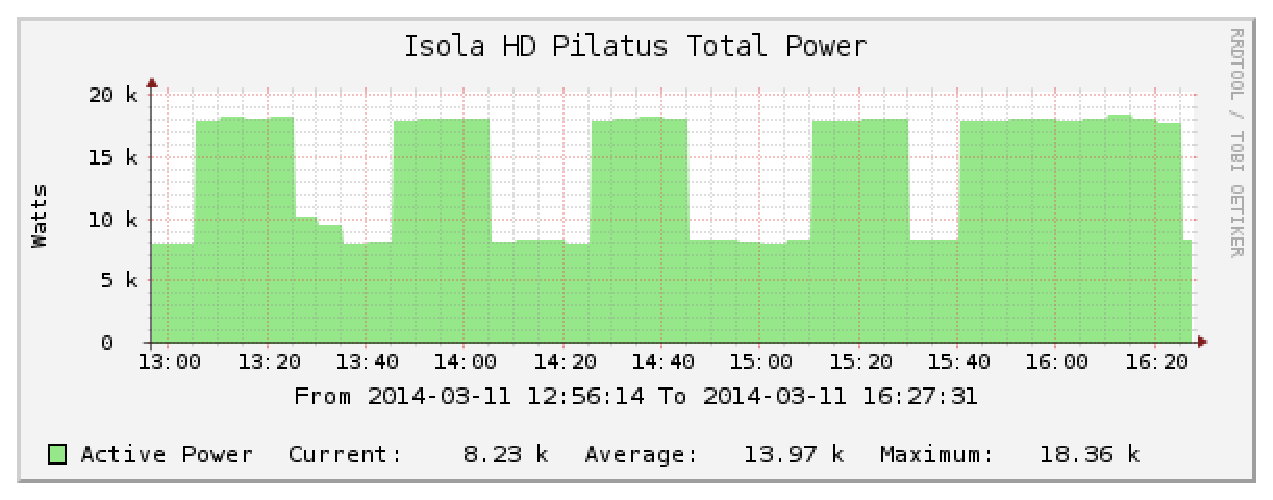
\includegraphics[width=0.48\textwidth]{Figs/NRJ_benchmark_Pilatus.eps}
    \caption{Pilatus: Isola HD Total Power}
    \label{fig:2}
  \end{center}
\end{figure}

Figures~\ref{fig:1} and  \ref{fig:2} account respectively  for Monch's
Isola E1  Rack 2  and Pilatus' Isola  HD total power  measurements for
1-day or 2-days simulations. On  the Intel Ivy Bridge EP based cluster
(i.e. Monch), the 1-day simulation  was issued only twice due to usage
restrictions. As time resolution was set to one update every 5 minutes
for  power sampling,  the average  power consumption  was  computed by
considering 6 values for each single  run.  On the Intel Xeon E5 based
cluster (i.e.   Pilatus), the 1-day  simulation was issued  four times
and a 2-days  run only once. Similarly, the  average power consumption
was computed by  considering 4 values for each single  1-day run and 9
values  for the  2-days  run. Corresponding  results  are gathered  in
Table~\ref{tab:3}.

\begin{table}[htbf]
  \begin{center}
    \caption{Average power consumption (W) of the platforms}
    \label{tab:3}
    \begin{tabular}{ccc}
      \hline\noalign{\smallskip}
      \textbf{Simulation time} & \textbf{Xeon E5} & \textbf{Ivy Bridge EP} \\
      \noalign{\smallskip}\hline\noalign{\smallskip}
      \textbf{1 day} & 18122.01417 & 12658.52278 \\ 
      & 17979.61083 & 12586.40833 \\
      & 18065.45167 & - \\
      & 17973.02833 & - \\
      \noalign{\smallskip}\hline\noalign{\smallskip}
      \textbf{2 days} & 17997.57815 & - \\
      \noalign{\smallskip}\hline
    \end{tabular}
  \end{center}
\end{table}

In Figure~\ref{fig:3}, we compare both time-to-solution (right y-axis)
and  energy-to-solution (left  y-axis) metrics  on both  platforms. As
expected,  Xeon  E5 outperforms  Ivy  Bridge  EP,  being roughly  1.3x
faster.   The reason for  that is  two-fold: (1)  it has  higher clock
frequency than Ivy  Bridge (2.6 GHz against 2.2 GHz),  and (2) it aims
at  computing   speed  regardless   to  energy  consumption.   In  our
experiments,  Ivy  Bridge   EP  showed  the  best  energy-to-solution,
reducing the energy consumption of Xeon E5 by approximately $7\%$.

\begin{figure}[htbf]
  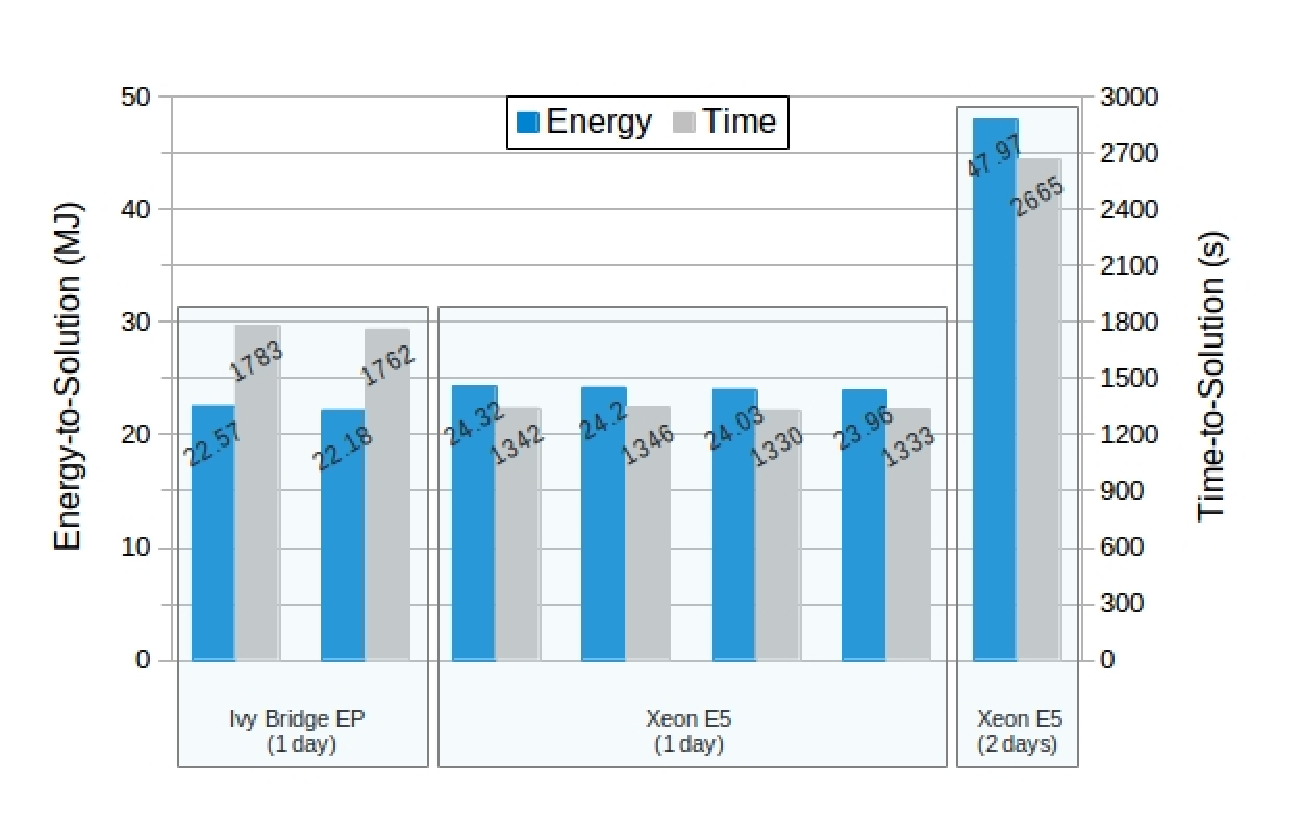
\includegraphics[width=0.5\textwidth]{Figs/Time_E2S_COSMO-ART.eps}
  \caption{Time-to-solution and  energy-to-solution comparison between
    Xeon E5 and Ivy Bridge-EP architectures}
  \label{fig:3}
\end{figure}
